% !TeX program = XeLaTeX
% !TeX root = ../pujavidhanam.tex

\setlength{\parindent}{0pt}
\chapt{श्री लक्ष्मी-कुबेर-पूजा}

\sect{पूर्वाङ्गविघ्नेश्वरपूजा}

(आचम्य)
\twolineshloka*
{शुक्लाम्बरधरं विष्णुं शशिवर्णं चतुर्भुजम्}
{प्रसन्नवदनं ध्यायेत् सर्वविघ्नोपशान्तये}
 
प्राणान्  आयम्य।  ॐ भूः + भूर्भुवः॒ सुव॒रोम्।
 
(अप उपस्पृश्य, पुष्पाक्षतान् गृहीत्वा)\\
ममोपात्तसमस्त दुरितक्षयद्वारा \\
श्रीपरमेश्वरप्रीत्यर्थं करिष्यमाणस्य कर्मणः\\
 निर्विघ्नेन परिसमाप्त्यर्थम् आदौ विघ्नेश्वरपूजां करिष्ये।

\twolineshloka*
{ॐ ग॒णानां᳚ त्वा ग॒णप॑तिꣳ हवामहे क॒विं क॑वी॒नामु॑प॒मश्र॑वस्तमम्}
{ज्ये॒ष्ठ॒राजं॒ ब्रह्म॑णां ब्रह्मणस्पत॒ आ नः॑ शृ॒ण्वन्नू॒तिभिः॑ सीद॒ साद॑नम्}
अस्मिन् हरिद्राबिम्बे महागणपतिं ध्यायामि, आवाहयामि।\\


ॐ महागणपतये नमः  आसनं समर्पयामि।\\
पादयोः पाद्यं समर्पयामि। हस्तयोरर्घ्यं समर्पयामि।\\
आचमनीयं समर्पयामि।\\
ॐ भूर्भुवस्सुवः। शुद्धोदकस्नानं समर्पयामि।\\
स्नानानन्तरमाचमनीयं समर्पयामि।\\
वस्त्रार्थमक्षतान् समर्पयामि।\\
यज्ञोपवीताभरणार्थे अक्षतान् समर्पयामि।\\
दिव्यपरिमलगन्धान् धारयामि।\\
गन्धस्योपरि हरिद्राकुङ्कुमं समर्पयामि। अक्षतान् समर्पयामि। \\
पुष्पमालिकां समर्पयामि। पुष्पैः पूजयामि।

\dnsub{अर्चना}
% \setenumerate{label=\devanumber.}
% \renewcommand{\labelenumi}{\devanumber\theenumi.}
\begin{enumerate}%[label=\devanumber\value{enumi}]
\begin{minipage}{0.475\linewidth}   
\item ॐ सुमुखाय नमः
\item ॐ एकदन्ताय नमः
\item ॐ कपिलाय नमः
\item ॐ गजकर्णकाय नमः
\item ॐ लम्बोदराय नमः
\item ॐ विकटाय नमः
\item ॐ विघ्नराजाय नमः
\item ॐ विनायकाय नमः
\item ॐ धूमकेतवे नमः
  \end{minipage}
  \begin{minipage}{0.525\linewidth}
\item ॐ गणाध्यक्षाय नमः
\item ॐ फालचन्द्राय नमः
\item ॐ गजाननाय नमः
\item ॐ वक्रतुण्डाय नमः
\item ॐ शूर्पकर्णाय नमः
\item ॐ हेरम्बाय नमः
\item ॐ स्कन्दपूर्वजाय नमः
\item ॐ सिद्धिविनायकाय नमः
\item ॐ विघ्नेश्वराय नमः
  \end{minipage}
\end{enumerate}
नानाविधपरिमलपत्रपुष्पाणि समर्पयामि॥\\
धूपमाघ्रापयामि।\\
अलङ्कारदीपं सन्दर्शयामि।\\
नैवेद्यम्।\\
ताम्बूलं समर्पयामि।\\
कर्पूरनीराजनं समर्पयामि।\\
कर्पूरनीराजनानन्तरमाचमनीयं समर्पयामि।\\
{वक्रतुण्डमहाकाय कोटिसूर्यसमप्रभ।}\\
{अविघ्नं कुरु मे देव सर्वकार्येषु सर्वदा॥}\\
प्रार्थनाः समर्पयामि।

अनन्तकोटिप्रदक्षिणनमस्कारान् समर्पयामि।\\
छत्त्रचामरादिसमस्तोपचारान् समर्पयामि।\\

 
\sect{प्रधान पूजा — श्रीमहालक्ष्मी-पूजा}

\twolineshloka*
{शुक्लाम्बरधरं विष्णुं शशिवर्णं चतुर्भुजम्}
{प्रसन्नवदनं ध्यायेत् सर्वविघ्नोपशान्तये}
 
प्राणान्  आयम्य।  ॐ भूः + भूर्भुवः॒ सुव॒रोम्।

\dnsub{सङ्कल्पः}

ममोपात्तसमस्तदुरितक्षयद्वारा श्रीपरमेश्वरप्रीत्यर्थं शुभे शोभने मुहूर्ते अद्यब्रह्मणः
द्वितीयपरार्द्धे श्वेतवराहकल्पे वैवस्वतमन्वन्तरे अष्टाविंशतितमे कलियुगे प्रथमे पादे
जम्बूद्वीपे भारतवर्षे भरतखण्डे मेरोः दक्षिणेपार्श्वे शकाब्दे अस्मिन् वर्तमाने व्यावहारिके
 प्रभवादि षष्टिसंवत्सराणां मध्ये (  )\see{app:samvatsara_names} नाम संवत्सरे दक्षिनायने 
शरद्-ऋतौ तुला-मासे कृष्णपक्षे अमावास्यायां शुभतिथौ
(इन्दु / भौम / बुध / गुरु / भृगु / स्थिर / भानु) वासरयुक्तायाम्
(  )\see{app:nakshatra_names} नक्षत्र (  )\see{app:yoga_names} नाम  योग  (चतुष्पात्/नागव) करण युक्तायां च एवं गुण विशेषण विशिष्टायाम्
अस्याम् अमावास्यायां शुभतिथौ 
अस्माकं सहकुटुम्बानां क्षेमस्थैर्य-धैर्य-वीर्य-विजय आयुरारोग्य ऐश्वर्याभिवृद्ध्यर्थम्
 धर्मार्थकाममोक्ष\-चतुर्विधफलपुरुषार्थसिद्ध्यर्थं पुत्रपौत्राभि\-वृद्ध्यर्थम् इष्टकाम्यार्थसिद्ध्यर्थम्
मम इहजन्मनि पूर्वजन्मनि जन्मान्तरे च सम्पादितानां ज्ञानाज्ञानकृतमहा\-पातकचतुष्टय
व्यतिरिक्तानां रहस्यकृतानां प्रकाशकृतानां सर्वेषां पापानां सद्य अपनोदनद्वारा सकल 
पापक्षयार्थं
श्रीमहालक्ष्मी-प्रीत्यर्थं श्रीमहालक्ष्मी-पूजां करिष्ये। तदङ्गं मातृगणपूजां नवग्रहपूजां लोकपाल-पूजां च करिष्ये। 
तदङ्गं कलशपूजां च करिष्ये। 


श्रीविघ्नेश्वराय नमः यथास्थानं प्रतिष्ठापयामि। शोभनार्थे क्षेमाय पुनरागमनाय च।\\
(गणपति प्रसादं शिरसा गृहीत्वा)

\dnsub{आसन-पूजा}
\centerline{पृथिव्या  मेरुपृष्ठ  ऋषिः।  सुतलं  छन्दः।  कूर्मो  देवता॥}
\twolineshloka*
{पृथ्वि  त्वया  धृता  लोका  देवि  त्वं  विष्णुना  धृता}
{त्वं  च  धारय  मां  देवि  पवित्रं  चाऽऽसनं  कुरु}


\dnsub{घण्टापूजा}
\twolineshloka*
{आगमार्थं तु देवानां गमनार्थं तु रक्षसाम्}
{घण्टारवं करोम्यादौ देवताऽऽह्वानकारणम्}


\dnsub{कलशपूजा}
ॐ कलशाय नमः दिव्यगन्धान् धारयामि।\\
ॐ गङ्गायै नमः। ॐ यमुनायै नमः। ॐ गोदावर्यै नमः।  ॐ सरस्वत्यै नमः। ॐ नर्मदायै नमः। ॐ सिन्धवे नमः। ॐ कावेर्यै नमः।\\
ॐ सप्तकोटिमहातीर्थान्यावाहयामि।\\[-0.25ex]

(अथ कलशं स्पृष्ट्वा जपं कुर्यात्) \\
आपो॒ वा इ॒द सर्वं॒ विश्वा॑ भू॒तान्याप॑ प्रा॒णा वा आप॑ प॒शव॒ आपो\-ऽन्न॒मापोऽमृ॑त॒माप॑ स॒म्राडापो॑ वि॒राडाप॑ स्व॒राडाप॒श्\-छन्दा॒स्यापो॒ ज्योती॒ष्यापो॒ यजू॒ष्याप॑ स॒त्यमाप॒ सर्वा॑ दे॒वता॒ आपो॒ भूर्भुव॒ सुव॒राप॒ ओम्॥\\

\twolineshloka* 
{कलशस्य मुखे विष्णुः कण्ठे रुद्रः समाश्रितः}
{मूले तत्र स्थितो ब्रह्मा मध्ये मातृगणाः स्मृताः}
\threelineshloka* 
{कुक्षौ तु सागराः सर्वे सप्तद्वीपा वसुन्धरा}
{ऋग्वेदोऽथ यजुर्वेदः सामवेदोऽप्यथर्वणः}
{अङ्गैश्च सहिताः सर्वे कलशाम्बुसमाश्रिताः}
\twolineshloka* 
{गङ्गे च यमुने चैव गोदावरि सरस्वति}
{नर्मदे सिन्धुकावेरि जलेऽस्मिन् सन्निधिं कुरु}
\twolineshloka*
{सर्वे समुद्राः सरितः तीर्थानि च ह्रदा नदाः}
{आयान्तु देवपूजार्थं दुरितक्षयकारकाः}

\centerline{ॐ भूर्भुवः॒ सुवो॒ भूर्भुवः॒ सुवो॒ भूर्भुवः॒ सुवः॑।}

(इति कलशजलेन सर्वोपकरणानि आत्मानं च प्रोक्ष्य।)


\dnsub{आत्म-पूजा}
ॐ आत्मने नमः, दिव्यगन्धान् धारयामि।
\begin{multicols}{2}
१. ॐ आत्मने नमः\\
२. ॐ अन्तरात्मने नमः\\
३. ॐ योगात्मने नमः\\
४. ॐ जीवात्मने नमः\\
५. ॐ परमात्मने नमः\\
६. ॐ ज्ञानात्मने नमः
\end{multicols}
समस्तोपचारान् समर्पयामि।

\twolineshloka*
{देहो देवालयः प्रोक्तो जीवो देवः सनातनः}
{त्यजेदज्ञाननिर्माल्यं सोऽहं भावेन पूजयेत्}


\begin{minipage}{\linewidth}
\dnsub{पीठ-पूजा}

\begin{multicols}{2}
\begin{enumerate}
\item ॐ आधारशक्त्यै नमः
\item ॐ मूलप्रकृत्यै नमः
\item ॐ आदिकूर्माय नमः 
\item ॐ आदिवराहाय नमः
\item ॐ अनन्ताय नमः
\item ॐ पृथिव्यै नमः
\item ॐ रत्नमण्डपाय नमः
\item ॐ रत्नवेदिकायै नमः
\item ॐ स्वर्णस्तम्भाय नमः
\item ॐ श्वेतच्छत्त्राय नमः
\item ॐ कल्पकवृक्षाय नमः
\item ॐ क्षीरसमुद्राय नमः 
\item ॐ सितचामराभ्यां नमः
\item ॐ योगपीठासनाय नमः
\end{enumerate}
\end{multicols}

\end{minipage}

\dnsub{गुरु ध्यानम्}

\twolineshloka*
{गुरुर्ब्रह्मा गुरुर्विष्णुर्गुरुर्देवो महेश्वरः}
{गुरुः साक्षात् परं ब्रह्म तस्मै श्री गुरवे नमः}


\sect{मातृगणपूजा}

\begin{enumerate}%[label=\devanumber\value{enumi}]
\begin{minipage}{0.475\linewidth}   
\item ॐ गौर्यै नमः
\item ॐ पद्मायै नमः
\item ॐ शच्यै नमः
\item ॐ मेधायै नमः
\item ॐ सावित्र्यै नमः
\item ॐ विजयायै नमः
\item ॐ जयायै नमः
\item ॐ देवसेनायै नमः
  \end{minipage}
  \begin{minipage}{0.525\linewidth}
\item ॐ स्वधायै नमः
\item ॐ स्वाहायै नमः
\item ॐ मातृभ्यो नमः
\item ॐ लोकमातृभ्यो नमः
\item ॐ धृत्यै नमः
\item ॐ पुष्ट्यै नमः
\item ॐ तुष्ट्यै नमः
\item ॐ आत्मनः कुलदेवतायै नमः
  \end{minipage}
\end{enumerate}

षोडश-मातृभ्यो नमः ध्यायामि। आवाहयामि। आसनं समर्पयामि।
पाद्यं समर्पयामि। अर्घ्यं समर्पयामि। आचमनीयं समर्पयामि। 
ॐ भूर्भुवस्सुवः। शुद्धोदकस्नानं समर्पयामि।\\
स्नानानन्तरमाचमनीयं समर्पयामि।\\
वस्त्रार्थमक्षतान् समर्पयामि।\\
आभरणार्थम् अक्षतान् समर्पयामि।\\
दिव्यपरिमलगन्धान् धारयामि।\\
गन्धस्योपरि हरिद्राकुङ्कुमं समर्पयामि। अक्षतान् समर्पयामि। \\
पुष्पमालिकां समर्पयामि।
धूपदीपार्थम् अक्षतान् समर्पयामि।\\

नैवेद्यम्। (कदलीफलानि)\\
कर्पूरताम्बूलं कर्पूरनीराजनार्थं अक्षतान् समर्पयामि।\\
प्रार्थनाः समर्पयामि।

\twolineshloka*
{आयुरारोग्यमैश्वर्यं ददध्वं मातरो मम}
{निर्विघ्नं सर्वकार्येषु कुरुध्वं सगणाधिपाः}

\twolineshloka*
{गौरी पद्मा शची मेधा सावित्री विजया जया}
{देवसेना स्वधा स्वाहा मातरो लोकमातरः}

\twolineshloka*
{धृतिः पुष्टिस्तथा तुष्टिरात्मनः कुलदेवता}
{गणेशेनाधिका ह्येता वरदाभयपाणयः}


अनन्तकोटिप्रदक्षिणनमस्कारान् समर्पयामि।\\
छत्त्रचामरादिसमस्तोपचारान् समर्पयामि।\\

% !TeX program = XeLaTeX
% !TeX root = ../pujavidhanam.tex
\sect{नवग्रहपूजा}

(चित्रे दर्शितवत् मण्डलानि प्रतिष्ठाप्य आरभेत।)

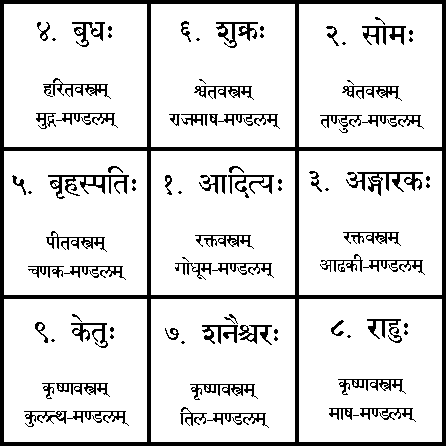
\includegraphics{purvanga/navagraha-diagram.pdf}

\twolineshloka
{जपाकुसुमसङ्काशं काश्यपेयं महद्युतिम्}
{तमोऽरिं सर्वपापघ्नं प्रणतोऽस्मि दिवाकरम्}

आ स॒त्येन॒ रज॑सा॒ वर्त॑मानो निवे॒शय॑न्न॒मृतं॒ मर्त्यं॑ च। हि॒र॒ण्यये॑न सवि॒ता रथे॒नाऽदे॒वो या॑ति॒
भुव॑ना वि॒पश्य\sn{}। अ॒ग्निं दू॒तं वृ॑णीमहे॒ होता॑रं वि॒श्ववे॑दसम्। अ॒स्य य॒ज्ञस्य॑ सु॒क्रतुम्॥
येषा॒मीशे॑ पशु॒पति॑ पशू॒नां चतु॑ष्पदामु॒त च॑ द्वि॒पदाम्। निष्क्री॑तो॒ऽयं य॒ज्ञियं॑ भा॒गमे॑तु
रा॒यस्पोषा॒ यज॑मानस्य सन्तु॥  अधिदेवता प्रत्यधिदेवता सहिताय आदित्याय॒ नम॥ 

अस्मिन् मण्डले अधिदेवता-प्रत्यधिदेवता-सहितं आदित्य-ग्रहं ध्यायामि। आवाहयामि।

\twolineshloka
{दधिशङ्खतुषाराभं क्षीरोदार्णवसम्भवम्}
{नमामि शशिनं सोमं शम्भोर्मुकुटभूषणम्}

आप्या॑यस्व॒ समे॑तु ते वि॒श्वत॑ सोम॒ वृष्णि॑यम्। भवा॒ वाज॑स्य सङ्ग॒थे॥ अ॒प्सु मे॒ सोमो॑
अब्रवीद॒न्तर्विश्वा॑नि भेष॒जा। अ॒ग्निं च॑ वि॒श्वश॑म्भुव॒माप॑श्च वि॒श्वभे॑षजीः। गौ॒री मि॑माय
सलि॒लानि॒ तक्ष॒ती। एक॑पदी द्वि॒पदी॒ सा चतु॑ष्पदी। अ॒ष्टाप॑दी॒ नव॑पदी बभू॒वुषी। स॒हस्राक्षरा पर॒मे
व्यो॑मन्।  अधिदेवता प्रत्यधिदेवता सहिताय सोमाय॒ नम॥ 

अस्मिन् मण्डले अधिदेवता-प्रत्यधिदेवता-सहितं सोम-ग्रहं ध्यायामि। आवाहयामि।


\twolineshloka
{धरणीगर्भसम्भूतं विद्युत्कान्तिसमप्रभम्}
{कुमारं शक्तिहस्तं च मङ्गलं प्रणमाम्यहम्}

अ॒ग्निर्मू॒र्द्धा दि॒वः क॒कुत्पति॑ पृथि॒व्या अ॒यम्। अ॒पा रेतासि जिन्वति। स्यो॒ना पृ॑थिवि॒
भवा॑ऽनृक्ष॒रा नि॒वेश॑नी। यच्छा॑न॒ शर्म॑ स॒प्रथा। क्षेत्र॑स्य॒ पति॑ना व॒य हि॒ते ने॑व जयामसि।
गामश्वं॑ पोषयि॒त्न्वा स नो॑ मृडाती॒दृशे॥  अधिदेवता प्रत्यधिदेवता सहिताय अङ्गारकाय॒ नम॥ 

अस्मिन् मण्डले अधिदेवता-प्रत्यधिदेवता-सहितं अङ्गारक-ग्रहं ध्यायामि। आवाहयामि।


\twolineshloka
{प्रियङ्गुकलिकाश्यामं रूपेणाप्रतिमं बुधम्}
{सौम्यं सौम्यगुणोपेतं तं बुधं प्रणमाम्यहम्}

उद्बु॑ध्यस्वाग्ने॒ प्रति॑जागृह्येनमिष्टापू॒र्ते ससृ॑जेथाम॒यं च॑। पुन॑ कृ॒ण्वस्त्वा॑ पि॒तरं॒
युवा॑नम॒न्वातासी॒त्वयि॒ तन्तु॑मे॒तम्॥ इ॒दं विष्णु॒र्विच॑क्रमे त्रे॒धा निद॑धे प॒दम्। समू॑ढमस्यपा
सु॒रे॥ विष्णो॑ र॒राट॑मसि॒ विष्णो पृ॒ष्ठम॑सि॒ विष्णो॒ श्नप्त्रेस्थो॒ विष्णो॒ स्यूर॑सि॒
विष्णोर्ध्रु॒वम॑सि वैष्ण॒वम॑सि॒ विष्ण॑वे त्वा।  अधिदेवता प्रत्यधिदेवता सहिताय बुधाय॒ नम॥ 

अस्मिन् मण्डले अधिदेवता-प्रत्यधिदेवता-सहितं बुध-ग्रहं ध्यायामि। आवाहयामि।


\twolineshloka
{देवानां च ऋषीणां च गुरुं काञ्चनसन्निभम्}
{बुद्धिभूतं त्रिलोकेशं तं नमामि बृहस्पतिम्}

बृह॑स्पते॒ अति॒यद॒र्यो अर्हाद्वि॒मद्वि॒भाति॒ क्रतु॑म॒ज्जने॑षु। यद्दी॒दय॒च्छव॑सर्त\-प्रजात॒
तद॒स्मासु॒ द्रवि॑णं धेहि चि॒त्रम्॥ इन्द्र॑मरुत्व इ॒ह पा॑हि॒ सोमं॒ यथा॑ शार्या॒ते अपि॑बः सु॒तस्य॑।
तव॒ प्रणी॑ती॒ तव॑ शूर॒शर्म॒न्नावि॑वासन्ति क॒वय॑ सुय॒ज्ञाः॥ ब्रह्म॑जज्ञा॒नं प्र॑थ॒मं
पु॒रस्ता॒द्विसी॑म॒तः सु॒रुचो॑ वे॒न आ॑वः। सबु॒ध्निया॑ उप॒मा अ॑स्य वि॒ष्ठाः स॒तश्च॒ योनि॒मस॑तश्च॒
विव॑॥ अधिदेवता प्रत्यधिदेवता सहिताय बृहस्पतये॒ नम॥ 

अस्मिन् मण्डले अधिदेवता-प्रत्यधिदेवता-सहितं बृहस्पति-ग्रहं ध्यायामि। आवाहयामि।

\twolineshloka
{हिमकुन्दमृणालाभं दैत्यानां परमं गुरुम्}
{सर्वशास्त्रप्रवक्तारं भार्गवं प्रणमाम्यहम्}

प्रव॑ शु॒क्राय॑ भा॒नवे॑ भरध्व ह॒व्यं म॒तिं चा॒ग्नये॒ सुपू॑तम्॥ यो दैव्या॑नि॒ मानु॑षा
ज॒नूष्य॒न्तर्विश्वा॑नि वि॒द्म ना॒ जिगा॑ति॥ इ॒न्द्रा॒णीमा॒सु नारि॑षु सु॒पत्नी॑म॒हम॑श्रवम्। न
ह्य॑स्या अप॒रञ्च॒न ज॒रसा॒ मर॑ते॒ पति॑॥ इन्द्रं॑ वो वि॒श्वत॒स्परि॒ हवा॑महे॒ जनेभ्यः। अ॒स्माक॑मस्तु॒
केव॑लः॥  अधिदेवता प्रत्यधिदेवता सहिताय शुक्राय॒ नम॥ 

अस्मिन् मण्डले अधिदेवता-प्रत्यधिदेवता-सहितं शुक्र-ग्रहं ध्यायामि। आवाहयामि।

\twolineshloka
{नीलाञ्जनसमाभासं रविपुत्रं यमाग्रजम्}
{छायामार्तण्डसम्भूतं तं नमामि शनैश्चरम्}

शं नो॑ दे॒वीर॒भिष्ट॑य॒ आपो॑ भवन्तु पी॒तये। शंयोर॒भिस्र॑वन्तु नः॥ प्रजा॑पते॒ न त्वदे॒तान्य॒न्यो
विश्वा॑ जा॒तानि॒ परि॒ता ब॑भूव। यत्का॑मास्ते जुहु॒मस्तन्नो॑ अस्तु व॒य स्या॑म॒ पत॑यो रयी॒णाम्। इ॒मं
य॑मप्रस्त॒रमाहि सीदाऽङ्गि॑रोभिः पि॒तृभि॑ संविदा॒नः। आत्वा॒ मन्त्रा कविश॒स्ता व॑हन्त्वे॒ना रा॑जन्
ह॒विषा॑ मादयस्व॥  अधिदेवता प्रत्यधिदेवता सहिताय शनैश्चराय॒ नम॥ 

अस्मिन् मण्डले अधिदेवता-प्रत्यधिदेवता-सहितं शनैश्चर-ग्रहं ध्यायामि। आवाहयामि।

\twolineshloka
{अर्धकायं महावीर्यं चन्द्रादित्यविमर्दनम्}
{सिंहिकागर्भसम्भूतं तं राहुं प्रणमाम्यहम्}

कया॑ नश्चि॒त्र आभु॑वदू॒ती स॒दावृ॑ध॒ सखा। कया॒ शचि॑ष्ठया वृ॒ता। आऽयङ्गौः
पृश्नि॑रक्रमी॒दस॑नन्मा॒तरं॒ पुन॑। पि॒तरं॑ च प्र॒यन्त्सुव॑। यत्ते॑ दे॒वी निर्ऋ॑तिराब॒बन्ध॒ दाम॑
ग्री॒वास्व॑विच॒र्त्यम्। इ॒दं  ते॒ तद्विष्या॒म्यायु॑षो॒ न मध्या॒दथा॑जी॒वः पि॒तुम॑द्धि॒ प्रमु॑क्तः॥ 
अधिदेवता प्रत्यधिदेवता सहिताय राहवे॒ नम॥ 

अस्मिन् मण्डले अधिदेवता-प्रत्यधिदेवता-सहितं राहु-ग्रहं ध्यायामि। आवाहयामि।

\twolineshloka
{पलाशपुष्पसङ्काशं तारकाग्रहमस्तकम्}
{रौद्रं रौद्रात्मकं घोरं तं केतुं प्रणमाम्यहम्}

के॒तुं कृ॒ण्वन्न॑के॒तवे॒ पेशो॑ मर्या अपे॒शसे। समु॒षद्भि॑रजायथाः॥ ब्र॒ह्मा दे॒वानां पद॒वीः
क॑वी॒नामृषि॒र्विप्रा॑णां महि॒षो मृ॒गाणाम्। श्ये॒नो गृध्रा॑णा॒ स्वधि॑ति॒र्वना॑ना॒ सोम॑
प॒वित्र॒मत्ये॑ति॒ रेभ\sn{}। (ऋक्) सचि॑त्र चि॒त्रं चि॒तयन् तम॒स्मे चित्र॑क्षत्र चि॒त्रत॑मं वयो॒धाम्।
च॒न्द्रं र॒यिं पु॑रु॒वीरं बृ॒हन्तं॒ चन्द्र॑च॒न्द्राभि॑र्गृण॒ते यु॑वस्व॥  अधिदेवता प्रत्यधिदेवता
सहिताय केतवे॒ नम॥ 

अस्मिन् मण्डले अधिदेवता-प्रत्यधिदेवता-सहितं केतु-ग्रहं ध्यायामि। आवाहयामि।

आदित्यादि नवग्रहदेवताभ्यो नमः आसनं समर्पयामि।
पाद्यं समर्पयामि। अर्घ्यं समर्पयामि। आचमनीयं समर्पयामि। 

शुद्धोदकस्नानं समर्पयामि। स्नानानन्तरम् आचमनीयं समर्पयामि।
वस्त्रार्थम् अक्षतान् समर्पयामि।\\
यज्ञोपवीताभरणार्थे अक्षतान् समर्पयामि।\\
दिव्यपरिमलगन्धान् धारयामि।\\
गन्धस्योपरि हरिद्राकुङ्कुमं समर्पयामि। अक्षतान् समर्पयामि। \\
पुष्पैः पूजयामि।

\begin{enumerate}%[label=\devanumber\value{enumi}]
\item ॐ आदित्याय नमः
\item ॐ अङ्गारकाय नम​:
\item ॐ शुक्राय नमः
\item ॐ सोमाय नम​:
\item ॐ बुधाय नम​:
\item ॐ बृहस्पतये नमः
\item ॐ शनैश्चराय नमः
\item ॐ राहवे नमः
\item ॐ केतवे नम​:
\end{enumerate}

नानाविध-परिमल-पत्र-पुष्पाणि समर्पयामि।

आदित्यादि नवग्रहदेवताभ्यो नमः धूपमाघ्रापयामि।\\
दीपं दर्शयामि।\\
नैवेद्यम्। \\
कर्पूरताम्बूलं समर्पयामि। कर्पूरनीराजनं दर्शयामि।\\
प्रार्थनाः समर्पयामि।
अनन्तकोटिप्रदक्षिणनमस्कारान् समर्पयामि।\\

आदित्यादि नवग्रहदेवताभ्यो नमः (अक्षतान् समर्पयित्वा) यथास्थानं प्रतिष्ठापयामि। शोभनार्थे क्षेमाय पुनरागमनाय च।


% !TeX program = XeLaTeX
% !TeX root = ..\pujavidhanam.tex

\sect{लोकपालपूजा}

प्राणान् आयम्य। ममोपात्तसमस्तदुरितक्षयद्वारा श्रीपरमेश्वरप्रीत्यर्थम् अद्य-पूर्वोक्त एवं गुण-विशेषेण विशिष्टायाम् अस्यां
अमावास्यायां शुभतिथौ श्रीमहालक्ष्मी-पूजाङ्गभूतां ब्रह्म-विष्णु-त्र्यम्बक-क्षेत्रपाल-पूजां करिष्ये।

अस्मिन् कूर्चे ब्रह्मादीन् ध्यायामि। ब्रह्मन् सरस्वत्या सह इह आगच्छ आगच्छ। सरस्वती-सहित-ब्रह्माणम् आवाहयामि। आसनं समर्पयामि।

लक्ष्मी-विष्णुभ्यां नमः।\\
ध्यायामि। आवाहयामि। आसनं समर्पयामि।

दुर्गा-त्र्यम्बकाभ्यां नमः।\\
ध्यायामि। आवाहयामि। आसनं समर्पयामि।

क्षेत्रपाल-भूमिभ्यां नमः।\\
ध्यायामि। आवाहयामि। आसनं समर्पयामि।

ब्रह्मादिभ्यो नमः पाद्यं समर्पयामि। अर्घ्यं समर्पयामि।
आचमनीयं समर्पयामि। शुद्धोदकस्नानं समर्पयामि। स्नानानन्तरम् आचमनीयं समर्पयामि।
वस्त्रार्थम् अक्षतान् समर्पयामि।
यज्ञोपवीताभरणार्थे अक्षतान् समर्पयामि।
दिव्यपरिमलगन्धान् धारयामि।
गन्धस्योपरि हरिद्राकुङ्कुमं समर्पयामि। अक्षतान् समर्पयामि। \\
पुष्पैः पूजयामि।\\

नैवेद्यम्। \\
कर्पूरताम्बूलं समर्पयामि। कर्पूरनीराजनं दर्शयामि।\\
प्रार्थनाः समर्पयामि।
अनन्तकोटिप्रदक्षिणनमस्कारान् समर्पयामि।\\

ब्रह्मादिभ्यो नमः (अक्षतान् समर्पयित्वा) यथास्थानं प्रतिष्ठापयामि। शोभनार्थे क्षेमाय पुनरागमनाय च।

\dnsub{प्रार्थना}

\twolineshloka*
{विघ्नराजं नमस्कृत्य नमस्कृत्य विधिं परम्}
{विष्णुं रुद्रं श्रियं दुर्गां वन्दे भक्त्या सरस्वतीम्}

\twolineshloka*
{क्षेत्राधिपं नमस्कृत्य दिवानाथं निशाकरम्}
{धरणीगर्भसम्भूतं शशिपुत्रं बृहस्पतिम्}

\twolineshloka*
{दैत्याचार्यं नमस्कृत्य सूर्यपुत्रं महाग्रहम्}
{राहुकेतू नमस्कृत्य यज्ञारम्भे विशेषतः}

\twolineshloka*
{शक्राद्या देवताः सर्वाः मुनींश्च प्रणमाम्यहम्}
{गर्गं मुनिं नमस्कृत्य नारदं मुनिसत्तमम्}

\twolineshloka*
{वसिष्ठं मुनिशार्दूलं विश्वामित्रं भृगोः सुतम्}
{व्यासं मुनिं नमस्कृत्य आचार्यांश्च तपोधनान्}

\twolineshloka*
{सर्वान् तान् प्रणमाम्येवं यज्ञरक्षाकरान् सदा}
{शङ्खचक्रगदाशार्ङ्ग-पद्मपाणिर्जनार्दनः}
\onelineshloka*
{सर्वासु दिक्षु रक्षेन्मां यावत् पूजावसानकम्}


\sect{षोडशोपचारपूजा}

\fourlineindentedshloka*
{अरुणकमलसंस्था तद्रजःपुञ्जवर्णा}
{करकमलधृतेष्टाऽभीतियुग्माम्बुजा च}
{मणिमकुटविचित्रालङ्कृता कल्पजातैः}
{भवतु भुवनमाता सन्ततं श्रीः श्रियै नः}

अस्मिन् बिम्बे श्रीमहालक्ष्मीं ध्यायामि।

\twolineshloka*
{आवाहये महालक्ष्मि चैतन्यस्तन्यदायिनि}
{विष्णुपत्नि जगन्मातः पूजां गृह्णीष्व ते नमः}
श्रीमहालक्ष्मीम् आवाहयामि।

\twolineshloka*
{तप्तकाञ्चनवर्णाभं मुक्तामणिविराजितम्}
{अमलं कमलं दिव्यम् आसनं प्रतिगृह्यताम्}
 आसनं समर्पयामि।\medskip


\twolineshloka*
{गङ्गातीर्थ-समुद्भूतं गन्ध-पुष्पादिभिर्युतम्}
{पाद्यं ददाम्यहं देवि गृहाणाऽऽशु नमोऽस्तु ते}
 पाद्यं समर्पयामि।\medskip

\twolineshloka*
{एलागन्धसमायुक्तं स्वर्णपात्रे प्रपूरितम्}
{अर्घ्यं गृहाण मद्दत्तं प्रसीद त्वं महेश्वरि}
 अर्घ्यं समर्पयामि।\medskip


\twolineshloka*
{सर्वलोकस्य या शक्तिः ब्रह्मरुद्रादिभिः स्तुता}
{ददाम्याचमनं तस्यै महालक्ष्म्यै मनोहरम्}
 आचमनीयं समर्पयामि।\medskip

घृतेन स्नपयामि। पुनः शुद्धोदकं समर्पयामि।\\
पयसा स्नपयामि। पुनः शुद्धोदकं समर्पयामि।\\
दध्ना स्नपयामि। पुनः शुद्धोदकं समर्पयामि।\\
मधुना स्नपयामि। पुनः शुद्धोदकं समर्पयामि।\\
पञ्चामृतेन स्नपयामि। पुनः शुद्धोदकं समर्पयामि।

(कलशजलेन श्री-सूक्तं जप्य) शुद्धोदकस्नानं समर्पयामि।
स्नानानन्तरम् आचमनीयं समर्पयामि।\medskip

\twolineshloka*
{दिव्याम्बरयुगं सूक्ष्मं कञ्चुकं च मनोहरम्}
{महालक्ष्मि महादेवि गृहाणेदं मयाऽर्पितम्}
 वस्त्रं समर्पयामि।\medskip

\twolineshloka*
{माङ्गल्यमणिसंयुक्तं मुक्ताविद्रुमसंयुतम्}
{दत्तं मङ्गलसूत्रं च गृहाण हरिवल्लभे}
कण्ठसूत्रं समर्पयामि।\medskip


\twolineshloka*
{रत्नकङ्कणवैडूर्य-मुक्ताहारादिकानि च}
{सुप्रसन्नेन मनसा दत्तानि त्वं गृहाण मे}
आभरणानि समर्पयामि।\medskip

\twolineshloka*
{सिन्दूरारुणवर्णा च सिन्दूरतिलकप्रिया}
{अतो दत्तं मया देवि सिन्दूरं प्रतिगृह्यताम्}
 तिलकं समर्पयामि। \medskip

\twolineshloka*
{मन्दार-पारिजाताद्याः पाटली केतकी तथा}
{माकन्दं कुरवं चैव गृहाणाऽऽशु नमोऽस्तु ते}
  पुष्पमालां धारयामि। 

\dnsub{अङ्गपूजा}
\begin{longtable}{ll@{— }l}
१.& ॐ चपलायै नमः & पादौ पूजयामि \\
२.& चञ्चलायै नमः & जानुनी पूजयामि\\
३.& कमलायै नमः & कटिं पूजयामि  \\
४.& कात्यायन्यै नमः & नाभिं पूजयामि\\
५.& जगन्मात्रे नमः & जठरं पूजयामि   \\
६.& विश्ववल्लभायै नमः & वक्षःस्थलं पूजयामि \\
७.& कमलवासिन्यै नमः & हस्तौ पूजयामि        \\
८.& पद्माननायै नमः & मुखं पूजयामि\\
९.& कमलपत्राक्ष्यै नमः & नेत्रत्रयं पूजयामि    \\
१०.& श्रियै नमः & शिरः पुजयामि\\
११.& महालक्ष्म्यै नमः & सर्वाणि अङ्गानि पूजयामि   \\
\end{longtable}

\dnsub{अष्टलक्ष्मी-अर्चना}
(प्राच्याम् आरभ्य अष्टदिक्षु प्रदक्षिणेन)

\begin{multicols}{2}
\begin{enumerate}
\item ॐ आद्यलक्ष्म्यै नमः
\item ॐ विद्यालक्ष्म्यै नमः
\item ॐ सौभाग्यलक्ष्म्यै नमः
\item ॐ अमृतलक्ष्म्यै नमः
\item ॐ कामलक्ष्म्यै नमः 
\item ॐ सत्यलक्ष्म्यै नमः
\item ॐ भोगलक्ष्म्यै नमः
\item ॐ योगलक्ष्म्यै नमः
\end{enumerate}
\end{multicols}

आद्यादिलक्ष्मीनां षोडशोपचारपूजार्थे पुष्पाणि समर्पयामि।

\dnsub{लक्ष्म्यष्टोत्तरशतनामावलिः}
\begin{multicols}{2}
\begin{flushleft}
ॐ प्रकृत्यै~नमः\\
ॐ विकृत्यै~नमः\\
ॐ विद्यायै~नमः\\
ॐ सर्वभूतहितप्रदायै~नमः\\
ॐ श्रद्धायै~नमः\\
ॐ विभूत्यै~नमः\\
ॐ सुरभ्यै~नमः\\
ॐ परमात्मिकायै~नमः\\
ॐ वाचे~नमः\\
ॐ पद्मालयायै~नमः\hfill\devanumber{10}\\
ॐ पद्मायै~नमः\\
ॐ शुचये~नमः\\
ॐ स्वाहायै~नमः\\
ॐ स्वधायै~नमः\\
ॐ सुधायै~नमः\\
ॐ धन्यायै~नमः\\
ॐ हिरण्मय्यै~नमः\\
ॐ लक्ष्म्यै~नमः\\
ॐ नित्यपुष्टायै~नमः\\
ॐ विभावर्यै~नमः\hfill\devanumber{20}\\
ॐ अदित्यै~नमः\\
ॐ दित्यै~नमः\\
ॐ दीप्तायै~नमः\\
ॐ वसुधायै~नमः\\
ॐ वसुधारिण्यै~नमः\\
ॐ कमलायै~नमः\\
ॐ कान्तायै~नमः\\
ॐ कामायै~नमः\\
ॐ क्षीरोदसम्भवायै~नमः\\
ॐ अनुग्रहपदायै~नमः\hfill\devanumber{30}\\
ॐ बुद्धये~नमः\\
ॐ अनघायै~नमः\\
ॐ हरिवल्लभायै~नमः\\
ॐ अशोकाममृतायै~नमः\\
ॐ दीप्तायै~नमः\\
ॐ लोकशोकविनाशिन्यै~नमः\\
ॐ धर्मनिलयायै~नमः\\
ॐ करुणायै~नमः\\
ॐ लोकमात्रे~नमः\\
ॐ पद्मप्रियायै~नमः\hfill\devanumber{40}\\
ॐ पद्महस्तायै~नमः\\
ॐ पद्माक्ष्यै~नमः\\
ॐ पद्मसुन्दर्यै~नमः\\
ॐ पद्मोद्भवायै~नमः\\
ॐ पद्ममुख्यै~नमः\\
ॐ पद्मनाभप्रियायै~नमः\\
ॐ रमायै~नमः\\
ॐ पद्ममालाधरायै~नमः\\
ॐ देव्यै~नमः\\
ॐ पद्मिन्यै~नमः\hfill\devanumber{50}\\
ॐ पद्मगन्धिन्यै~नमः\\
ॐ पुण्यगन्धायै~नमः\\
ॐ सुप्रसन्नायै~नमः\\
ॐ प्रसादाभिमुख्यै~नमः\\
ॐ प्रभायै~नमः\\
ॐ चन्द्रवदनायै~नमः\\
ॐ चन्द्रायै~नमः\\
ॐ चन्द्रसहोदर्यै~नमः\\
ॐ चतुर्भुजायै~नमः\\
ॐ चन्द्ररूपायै~नमः\hfill\devanumber{60}\\
ॐ इन्दिरायै~नमः\\
ॐ इन्दुशीतलायै~नमः\\
ॐ आह्लादजनन्यै~नमः\\
ॐ पुष्ट्यै~नमः\\
ॐ शिवायै~नमः\\
ॐ शिवकर्यै~नमः\\
ॐ सत्यै~नमः\\
ॐ विमलायै~नमः\\
ॐ विश्वजनन्यै~नमः\\
ॐ तुष्ट्यै~नमः\hfill\devanumber{70}\\
ॐ दारिद्र्यनाशिन्यै~नमः\\
ॐ प्रीतिपुष्करिण्यै~नमः\\
ॐ शान्तायै~नमः\\
ॐ शुक्लमाल्याम्बरायै~नमः\\
ॐ श्रियै~नमः\\
ॐ भास्कर्यै~नमः\\
ॐ बिल्वनिलयायै~नमः\\
ॐ वरारोहायै~नमः\\
ॐ यशस्विन्यै~नमः\\
ॐ वसुन्धरायै~नमः\hfill\devanumber{80}\\
ॐ उदाराङ्गायै~नमः\\
ॐ हरिण्यै~नमः\\
ॐ हेममालिन्यै~नमः\\
ॐ धनधान्यकर्यै~नमः\\
ॐ सिद्ध्यै~नमः\\
ॐ स्त्रैणसौम्यायै~नमः\\
ॐ शुभप्रदायै~नमः\\
ॐ नृपवेश्मगतानन्दायै~नमः\\
ॐ वरलक्ष्म्यै~नमः\\
ॐ वसुप्रदायै~नमः\hfill\devanumber{90}\\
ॐ शुभायै~नमः\\
ॐ हिरण्यप्राकारायै~नमः\\
ॐ समुद्रतनयायै~नमः\\
ॐ जयायै~नमः\\
ॐ मङ्गलायै~नमः\\
ॐ देव्यै~नमः\\
ॐ विष्णुवक्षःस्थलस्थितायै~नमः\\
ॐ विष्णुपत्न्यै~नमः\\
ॐ प्रसन्नाक्ष्यै~नमः\\
ॐ नारायणसमाश्रितायै~नमः\hfill\devanumber{100}\\
ॐ दारिद्र्यध्वंसिन्यै~नमः\\
ॐ देव्यै~नमः\\
ॐ सर्वोपद्रवहारिण्यै~नमः\\
ॐ नवदुर्गायै~नमः\\
ॐ महाकाल्यै~नमः\\
ॐ ब्रह्मविष्णुशिवात्मिकायै~नमः\\
ॐ त्रिकालज्ञानसम्पन्नायै~नमः\\
ॐ भुवनेश्वर्यै~नमः\\
\end{flushleft}
\end{multicols}

\sect{उत्तराङ्गपूजा}
\twolineshloka*
{वनस्पति-रसोत्पन्नो गन्धाढ्यो गन्ध उत्तमः}
{आघ्रेयः सर्वदेवानां धूपोऽयं प्रतिगृह्यताम्}
श्री महालक्ष्म्यै नमः धूपमाघ्रापयामि।\\
 
\twolineshloka*
{कार्पासवर्तिसंयुक्तं घृतयुक्तं मनोहरम्}
{तमोनाशकरं दीपं गृहाण परमेश्वर}
श्री महालक्ष्म्यै नमः अलङ्कारदीपं सन्दर्शयामि ।\\

\twolineshloka*
{नैवेद्यं गृह्यतां लक्ष्मि भक्ष्य-भोज्य-समन्वितम्}
{षड्रसैर्रचितं दिव्यं लक्ष्मीदेवि नमोऽस्तु ते}
नैवेद्यम्\\
- श्री महालक्ष्म्यै नमः (	) निवेदयामि, \\
अमृतापिधानमसि। निवेदनानन्तरम् आचमनीयं समर्पयामि।\\

पूगीफलसमायुक्तं नागवल्लीदलैर्युतम्।\\
कर्पूरचूर्णसंयुक्तं ताम्बूलं प्रतिगृह्यताम्॥\\
श्री महालक्ष्म्यै नमः कर्पूरताम्बूलं समर्पयामि।\\

श्री महालक्ष्म्यै नमः समस्त अपराध क्षमापनार्थं कर्पूरनीराजनं दर्शयामि।\\
कर्पूरनीरजनानन्तरम् आचमनीयं समर्पयामि।\\

 यो॑ऽपां पुष्पं॒ वेद॑। पुष्प॑वान् प्र॒जावान् पशु॒मान् भ॑वति।\\
च॒न्द्रमा॒ वा अ॒पां पुष्पम्। पुष्प॑वान् प्र॒जावान् पशु॒मान् भ॑वति।\\
य ए॒वं वेद॑। यो॑ऽपामा॒यत॑नं॒ वेद॑। आ॒यत॑नवान् भवति।\\

ओं तद्ब्र॒ह्म। ओं तद्वा॒युः। ओं तदा॒त्मा। ओं᳚ तथ्स॒त्यम्‌।\\
ओं᳚ तथ्सर्वम्᳚‌। ओं तत्पुरो॒र्नमः॥\\

अन्तश्चरति॑ भूते॒षु॒ गुहायां वि॑श्वमू॒र्तिषु। \\
त्वं यज्ञस्त्वं वषट्कारस्त्वमिन्द्रस्त्व रुद्रस्त्वं विष्णुस्त्वं ब्रह्म त्वं॑ प्रजा॒पतिः। \\
त्वं त॑दाप॒ आपो॒ ज्योती॒ रसो॒ऽमृतं॒ ब्रह्म॒ भूर्भुव॒स्सुव॒रोम्‌॥\\

श्री महालक्ष्म्यै नमः वेदोक्तमन्त्रपुष्पाञ्जलिं समर्पयामि।\\

स्वर्णपुष्पं समर्पयामि\\
 
अनन्तकोटिप्रदक्षिणनमस्कारान् समर्पयामि\\

छत्त्रचामरादिसमस्तोपचारान् समर्पयामि\\

हिरण्यगर्भगर्भस्थं हेमबीजं विभावसोः।\\
अनन्तपुण्यफलदम् अतः शान्तिं प्रयच्छ मे॥\\

आश्वयुज-अमावास्या-पुण्यकालेऽस्मिन् मया क्रियमाण श्रीमहालक्ष्मी-पूजायां
यद्देयमुपायनदानं तत्प्रतिनिधित्वेन हिरण्यं श्री महालक्ष्मीप्रीतिं
कामयमानः मनसोद्दिष्टाय ब्राह्मणाय सम्प्रददे नमः न मम। 
अनया पूजया श्री महालक्ष्मीः प्रीयताम्। 

\sect{ईशानादि पूजा}

\sect{कुबेर पूजा}



\dnsub{कुबेराष्टोत्तरशतनामावलिः}

\fourlineindentedshloka*
{मनुजबाह्यविमानवरस्तुतम्}
{गरुडरत्ननिभं निधिनायकम्}
{शिवसखं मुकुटादिविभूषितम्}
{वररुचिं तमहमुपास्महे सदा}

\twolineshloka*
{अगस्त्य देवदेवेश मर्त्यलोकहितेच्छया}
{पूजयामि विधानेन प्रसन्नसुमुखो भव}
\begin{multicols}{2}
\begin{flushleft}
ॐ कुबेराय नमः\\
ॐ धनदाय नमः\\
ॐ श्रीमते नमः\\
ॐ यक्षेशाय नमः\\
ॐ गुह्यकेश्वराय नमः\\
ॐ निधीशाय नमः\\
ॐ शङ्करसखाय नमः\\
ॐ महालक्ष्मीनिवासभुवे नमः\\
ॐ महापद्मनिधीशाय नमः\\
ॐ पूर्णाय नमः\hfill\devanumber{10}\\ %१०
ॐ पद्मनिधीश्वराय नमः\\
ॐ शङ्खाख्यनिधिनाथाय नमः\\
ॐ मकराख्यनिधिप्रियाय नमः\\
ॐ सुकच्छपाख्यनिधीशाय नमः\\
ॐ मुकुन्दनिधिनायकाय नमः\\
ॐ कुन्दाख्यनिधिनाथाय नमः\\
ॐ नीलनित्याधिपाय नमः\\
ॐ महते नमः\\
ॐ वरनिधिदीपाय नमः\\
ॐ पूज्याय नमः\hfill\devanumber{20}\\ %२०
ॐ लक्ष्मीसाम्राज्यदायकाय नमः\\
ॐ इलपिलापत्याय नमः\\
ॐ कोशाधीशाय नमः\\
ॐ कुलोचिताय नमः\\
ॐ अश्वारूढाय नमः\\
ॐ विश्ववन्द्याय नमः\\
ॐ विशेषज्ञाय नमः\\
ॐ विशारदाय नमः\\
ॐ नलकूबरनाथाय नमः\\
ॐ मणिग्रीवपित्रे नमः\hfill\devanumber{30}\\ %३०
ॐ गूढमन्त्राय नमः\\
ॐ वैश्रवणाय नमः\\
ॐ चित्रलेखामनःप्रियाय नमः\\
ॐ एकपिनाकाय नमः\\
ॐ अलकाधीशाय नमः\\
ॐ पौलस्त्याय नमः\\
ॐ नरवाहनाय नमः\\
ॐ कैलासशैलनिलयाय नमः\\
ॐ राज्यदाय नमः\\
ॐ रावणाग्रजाय नमः\hfill\devanumber{40}\\ %४०
ॐ चित्रचैत्ररथाय नमः\\
ॐ उद्यानविहाराय नमः\\
ॐ विहारसुकुतूहलाय नमः\\
ॐ महोत्सहाय नमः\\
ॐ महाप्राज्ञाय नमः\\
ॐ सदापुष्पकवाहनाय नमः\\
ॐ सार्वभौमाय नमः\\
ॐ अङ्गनाथाय नमः\\
ॐ सोमाय नमः\\
ॐ सौम्यादिकेश्वराय नमः\hfill\devanumber{50}\\ %५०
ॐ पुण्यात्मने नमः\\
ॐ पुरुहुतश्रियै नमः\\
ॐ सर्वपुण्यजनेश्वराय नमः\\
ॐ नित्यकीर्तये नमः\\
ॐ निधिवेत्रे नमः\\
ॐ लङ्काप्राक्तननायकाय नमः\\
ॐ यक्षिणीवृताय नमः\\
ॐ यक्षाय नमः\\
ॐ परमशान्तात्मने नमः\\
ॐ यक्षराजे नमः\hfill\devanumber{60}\\ %६०
ॐ यक्षिणीहृदयाय नमः\\ 
ॐ किन्नरेश्वराय नमः\\
ॐ किम्पुरुषनाथाय नमः\\
ॐ खड्गायुधाय नमः\\
ॐ वशिने नमः\\
ॐ ईशानदक्षपार्श्वस्थाय नमः\\
ॐ वायुवामसमाश्रयाय नमः\\
ॐ धर्ममार्गनिरताय नमः\\
ॐ धर्मसम्मुखसंस्थिताय नमः\\
ॐ नित्येश्वराय नमः\hfill\devanumber{70}\\ %७०
ॐ धनाध्यक्षाय नमः\\
ॐ अष्टलक्ष्म्याश्रितालयाय नमः\\
ॐ मनुष्यधर्मिणे नमः\\
ॐ सुकृतिने नमः\\
ॐ कोषलक्ष्मीसमाश्रिताय नमः\\
ॐ धनलक्ष्मीनित्यवासाय नमः\\
ॐ धान्यलक्ष्मीनिवासभुवे नमः\\
ॐ अष्टलक्ष्मीसदावासाय नमः\\
ॐ गजलक्ष्मीस्थिरालयाय नमः\\
ॐ राज्यलक्ष्मीजन्मगेहाय नमः\hfill\devanumber{80}\\ %८०
ॐ धैर्यलक्ष्मीकृपाश्रयाय नमः\\
ॐ अखण्डैश्वर्यसंयुक्ताय नमः\\
ॐ नित्यानन्दाय नमः\\
ॐ सुखाश्रयाय नमः\\
ॐ नित्यतृप्ताय नमः\\
ॐ निराशाय नमः\\
ॐ निरुपद्रवाय नमः\\
ॐ नित्यकामाय नमः\\
ॐ निराकाङ्क्षाय नमः\\
ॐ निरूपाधिकवासभुवे नमः\hfill\devanumber{90}\\ %९०
ॐ शान्ताय नमः\\
ॐ सर्वगुणोपेताय नमः\\
ॐ सर्वज्ञाय नमः\\
ॐ सर्वसम्मताय नमः\\
ॐ सर्वाणिकरुणापात्राय नमः\\
ॐ सदानन्दकृपालयाय नमः\\
ॐ गन्धर्वकुलसंसेव्याय नमः\\
ॐ सौगन्धिककुसुमप्रियाय नमः\\
ॐ स्वर्णनगरीवासाय नमः\\
ॐ निधिपीठसमाश्रयाय नमः\hfill\devanumber{100}\\ %१००
ॐ महामेरूत्तरस्थाय नमः\\
ॐ महर्षिगणसंस्तुताय नमः\\
ॐ तुष्टाय नमः\\
ॐ शूर्पणखाज्येष्ठाय नमः\\
ॐ शिवपूजारताय नमः\\
ॐ अनघाय नमः\\
ॐ राजयोगसमायुक्ताय नमः\\
ॐ राजशेखरपूज्याय नमः\\
ॐ राजराजाय नमः\\ %१०९
\end{flushleft}
\end{multicols}


\sect{प्रार्थना}
\sect{अपराध-क्षमापनम्}